% Created 2018-12-14 Fri 20:25
\documentclass[11pt]{article}
\usepackage[utf8]{inputenc}
\usepackage{lmodern}
\usepackage[T1]{fontenc}
\usepackage{fixltx2e}
\usepackage{graphicx}
\usepackage{longtable}
\usepackage{float}
\usepackage{wrapfig}
\usepackage{rotating}
\usepackage[normalem]{ulem}
\usepackage{amsmath}
\usepackage{textcomp}
\usepackage{marvosym}
\usepackage{wasysym}
\usepackage{amssymb}
\usepackage{amsmath}
\usepackage[version=3]{mhchem}
\usepackage[numbers,super,sort&compress]{natbib}
\usepackage{natmove}
\usepackage{url}
\usepackage{minted}
\usepackage{underscore}
\usepackage[linktocpage,pdfstartview=FitH,colorlinks,
linkcolor=blue,anchorcolor=blue,
citecolor=blue,filecolor=blue,menucolor=blue,urlcolor=blue]{hyperref}
\usepackage{attachfile}
\author{UH Computational Catalysis and Interface Chemistry Group}
\date{2016-09}
\title{Tutorials - For the Old and the New}
\begin{document}

\tableofcontents


\section{Introduction}
\label{sec-1}
The aim of this document is to help users who are new to the concepts and tools used in the group. By the end of this tutorial, the reader will should have a basic understanding of the various components of typical computational research workflows, starting from basic Linux commands to running calculations using VASP and other softwares. This document was not designed to be a thorough guide and the user is encourage to complement the information provided here with extensive Google searches.

We also recommend you to look at John Kitchin's \href{http://kitchingroup.cheme.cmu.edu/dft-book/dft.pdf}{DFT Book (pdf)} or \href{http://kitchingroup.cheme.cmu.edu/dft-book/dft.html}{html} versions since it contains many working examples that touch upon practical concepts of computational catalysis which can be easily (or relatively easy) followed and implemented.

\section{High Performance Computing}
\label{sec-2}
A significant portion of the research conducted in the group pertains to computational modeling in which various properties of interest for a system are calculated by means of \emph{ab initio} density functional theory calculations. We refer the reader to an excellent \href{https://www.wiley.com/en-us/Density+Functional+Theory\%3A+A+Practical+Introduction-p-9780470373170}{book} that elaborates on the nuts and bolts of DFT by Dr. David Sholl. These calculations are computationally intensive and are exclusively performed on computing clusters or supercomputers. These massively-parallel machines are accessed remotely through the \href{https://www.ssh.com/ssh/protocol/}{Secure Shell Protocol}, and the user is able to access his or her account on that machine. Once logged in, the user sets up these jobs and submits them to the system's resource manager, or the queue. Once resources become available, the queue executes the job and the user is notified upon completion of the job.

\subsection{Queues}
\label{sec-2-1}
The queue is a utility that accepts job submissions from users, implements a fair use policy, and allocates resources based on job requirements and other parameters. Most of the systems used by our group are managed by the \href{http://slurm.schedmd.com/}{=SLURM} Workload Manager=. Maxwell is managed by the \href{http://www.adaptivecomputing.com/products/open-source/torque/}{\texttt{Torque Resource Manager}}. The configuration keywords and parameters are different for different systems and every job submission script must contain these parameters for it to be accepted by the queue. The queue keywords are

For \texttt{SLURM}
\begin{minted}[frame=lines,fontsize=\scriptsize,linenos]{sh}
#SBATCH -p <queue partition>
#SBATCH -o myMPI.o%j
#SBATCH -N <number of nodes> -n <number of processors per node>
#SBATCH -t <walltime in hhh:mm:ss>
#SBATCH --mail-type=END
#SBATCH --mail-user=<user email id>
\end{minted}

A more detailed explanation of these parameters follows:
\begin{itemize}
\item queue partition: This specifies the partition to which you want to submit your job.
\item number of nodes: A node is a group of processors, which are designed to work together with maximum efficiency. A simple example of a node would be a computer with an Intel i5 processor, where the single node has 4 processors.
\item number of processors: This is the number of processors or threads in a node. Usually, the user is expected to request all processors in a node. This parameter is system configuration dependent.
\item walltime in hours: This specifies the time until which the job will execute on the system. Once runtime exceeds this value, the job execution is terminated.
\end{itemize}

\subsection{Jobscripts}
\label{sec-2-2}
Jobscripts are executable files of a defined environment which consist of executable code. Jobscripts can be in a variety of file formats and the most commonly used ones are python, shell and cshell jobscripts.
A jobscript and a simple file are differentiated by the file type identifier. This line tells the compiler, interpreter and any text-editor the type of the file. This removes the need for an extension to the file, which can also serve as an identifier. A properly identified file also enables source code formatting on text-editors.

An example python jobscript is  as follows
\begin{minted}[frame=lines,fontsize=\scriptsize,linenos]{sh}
#!/usr/bin/env python --> File environment identifier

#SBATCH -p batch
#SBATCH -o myMPI.o%j
#SBATCH -N 5 -n 100                            [SLURM Parameters]
#SBATCH -t 168:00:00
#SBATCH --mail-type=END
#SBATCH --mail-user=hthirumalai@gmail.com

# Your executable python code begins here
from ase.io import read
from ase.calculators.vasp import Vasp

...
\end{minted}

\begin{minted}[frame=lines,fontsize=\scriptsize,linenos]{sh}
#!/usr/bin/env python

#PBS -e stderr
#PBS -o stdout
#PBS -m ae
#PBS -M hthirumalai@gmail.com
#PBS -l walltime=100:00:00
#PBS -r n
#PBS -l nodes=1:ppn=12
#PBS -l pmem=2500mb
#PBS -S /bin/tcsh
#PBS -V

from ase import *
from ase.calculators.vasp import Vasp

...
\end{minted}

An example shell jobscript is
\begin{minted}[frame=lines,fontsize=\scriptsize,linenos]{sh}
#!/bin/sh --> File environment identifier

#SBATCH -p batch
#SBATCH -o myMPI.o%j
#SBATCH -N 5 -n 100                            [SLURM Parameters]
#SBATCH -t 168:00:00
#SBATCH --mail-type=END
#SBATCH --mail-user=hthirumalai@gmail.com

# Your executable shell script begins here
echo 'VASP starting execution ..'

...
\end{minted}

\begin{minted}[frame=lines,fontsize=\scriptsize,linenos]{sh}
#!/bin/sh

#PBS -e stderr
#PBS -o stdout
#PBS -m ae
#PBS -M mayerzmytm@gmail.com
#PBS -l walltime=100:00:00
#PBS -r n
#PBS -l nodes=1:ppn=12
#PBS -l pmem=2500mb
#PBS -S /bin/tcsh
#PBS -V

# Your executable shell script begins here
echo 'VASP starting execution ..'
\end{minted}

\subsection{System Specific Settings}
\label{sec-2-3}
Our group has access to various clusters at any given time and job scripts must be modified such that they execute without errors when transferred from one cluster to another. This section consists of all cluster relevant information. All storage-intensive jobs must be executed on the group's project directories. These locations are backed-up on a daily basis. \$SCRATCH directories on Cori and Stampede2 are short term, high I/O performance storage that are periodically purged. Therefore, the reader is advised to use these directories for running jobs only and transfer these files to permanent storage on the University of Houston clusters.

Opuntia
\begin{minted}[frame=lines,fontsize=\scriptsize,linenos]{sh}
project directory: /project/grabow

#SBATCH -p grabow
#SBATCH -o myMPI.o%j   
#SBATCH -N 1 -n 20
#SBATCH -t 24:00:00
#SBATCH --mail-type=END
#SBATCH --mail-user=@gmail.com
\end{minted}

uHPC
\begin{minted}[frame=lines,fontsize=\scriptsize,linenos]{sh}
project directory: /uhpc/grabow

#SBATCH -p batch
#SBATCH -o myMPI.o%j   
#SBATCH -N 1 -n 20
#SBATCH -t 24:00:00
#SBATCH --mail-type=END
#SBATCH --mail-user=@gmail.com
\end{minted}

Juniper
\begin{minted}[frame=lines,fontsize=\scriptsize,linenos]{sh}
project directory: /project/grabow

#SBATCH -p batch
#SBATCH -o myMPI.o%j   
#SBATCH -N 1 -n 24
#SBATCH -t 24:00:00
#SBATCH --mail-type=END
#SBATCH --mail-user=@gmail.com
\end{minted}

Sabine
\begin{minted}[frame=lines,fontsize=\scriptsize,linenos]{sh}
project directory: /brazos/grabow

#SBATCH -p batch
#SBATCH -o myMPI.o%j   
#SBATCH -N 1 -n 24
#SBATCH -t 24:00:00
#SBATCH --mail-type=END
#SBATCH --mail-user=@gmail.com
\end{minted}

Cori
\begin{minted}[frame=lines,fontsize=\scriptsize,linenos]{sh}
scratch directory: $SCRATCH
project directory: /global/project/projectdirs/m2029/

#SBATCH -p regular
#SBATCH -C knl
#SBATCH -A m2029
#SBATCH -o myMPI.o%j   
#SBATCH -N 1 -n 64
#SBATCH -t 24:00:00
#SBATCH --mail-type=END
#SBATCH --mail-user=@gmail.com  

AND

#SBATCH -p regular
#SBATCH -C haswell
#SBATCH -A m2029
#SBATCH -o myMPI.o%j   
#SBATCH -N 1 -n 32
#SBATCH -t 24:00:00
#SBATCH --mail-type=END
#SBATCH --mail-user=@gmail.com
\end{minted}

Stampede2
\begin{minted}[frame=lines,fontsize=\scriptsize,linenos]{sh}
scratch directory: $SCRATCH
project directory: $WORK

#SBATCH -p normal
#SBATCH -o myMPI.o%j   
#SBATCH -N 1 -n 64
#SBATCH -t 24:00:00
#SBATCH --mail-type=END
#SBATCH --mail-user=@gmail.com  

AND

#SBATCH -p skx-normal
#SBATCH -o myMPI.o%j   
#SBATCH -N 1 -n 48
#SBATCH -t 24:00:00
#SBATCH --mail-type=END
#SBATCH --mail-user=@gmail.com
\end{minted}

\subsection{Terminals}
\label{sec-2-4}
The terminal is the window that allows the user to interact with the computer through the command line. Any output from code can also be piped out to the command line on the terminal.

A Windows user needs to download software that provides a terminal for remote ssh access and Linux and Mac OS users can use the pre-installed terminal on their computer. The figure that follows shows a typical terminal window on a Mac OS computer. Users can access the terminals by searching for \texttt{Terminal} in Apple's Spotlight Search (command+space).

\begin{figure}[htb]
\centering
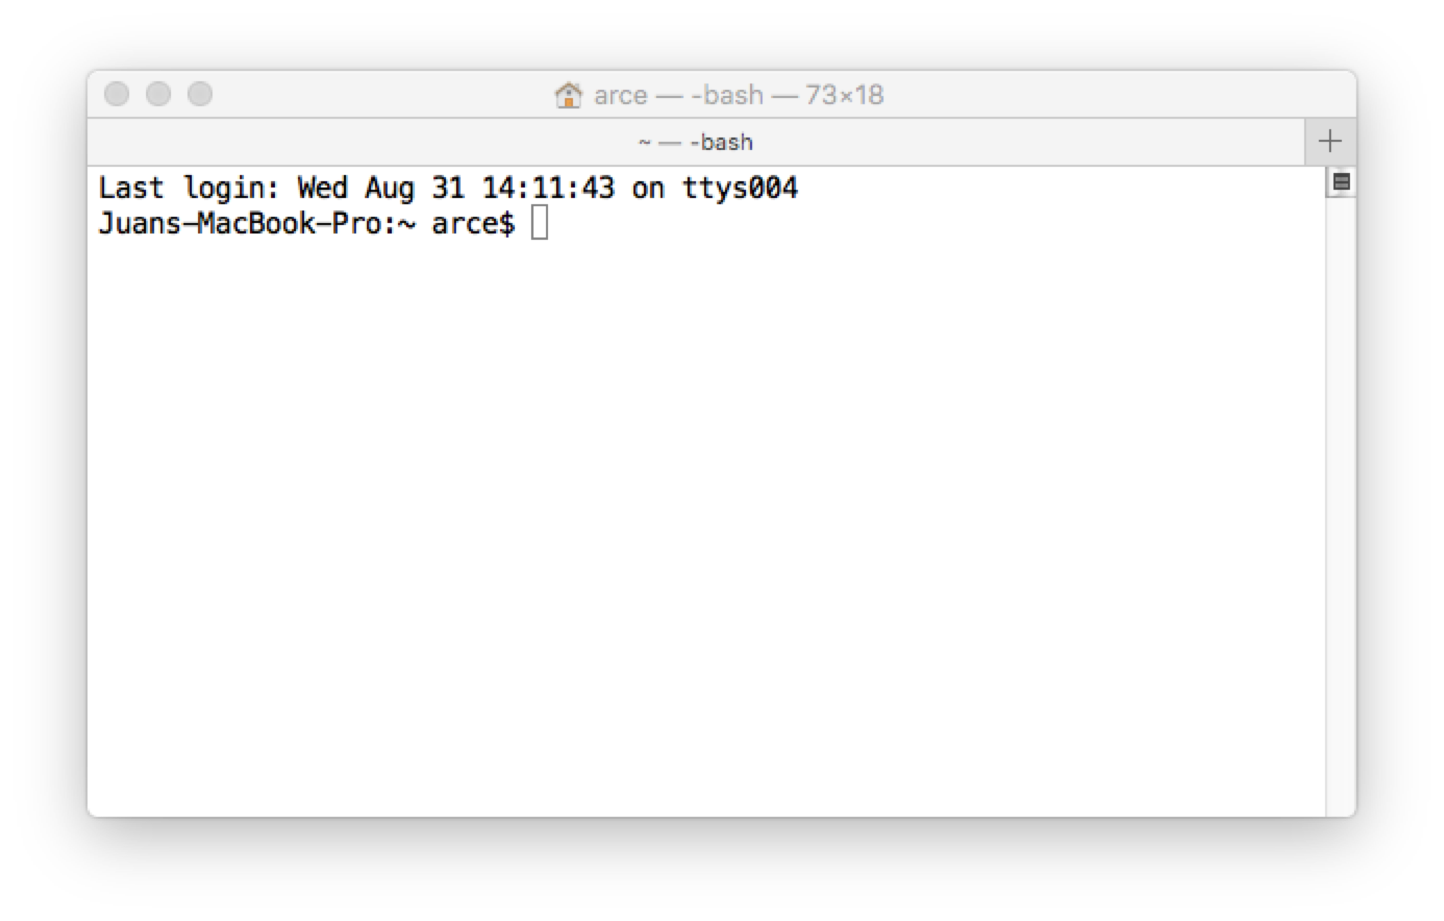
\includegraphics[width=.9\linewidth]{./figures/terminal-mac.png}
\caption{Terminal window on Mac OS}
\end{figure}

If you are a Linux user then you should be able to start a terminal without the need for any installation. Terminal on a Linux system running Ubuntu can be accessed using Ctrl+Alt+T. Multiple tabs can be opened by hitting Ctrl+Shift+T.
\begin{figure}[htb]
\centering
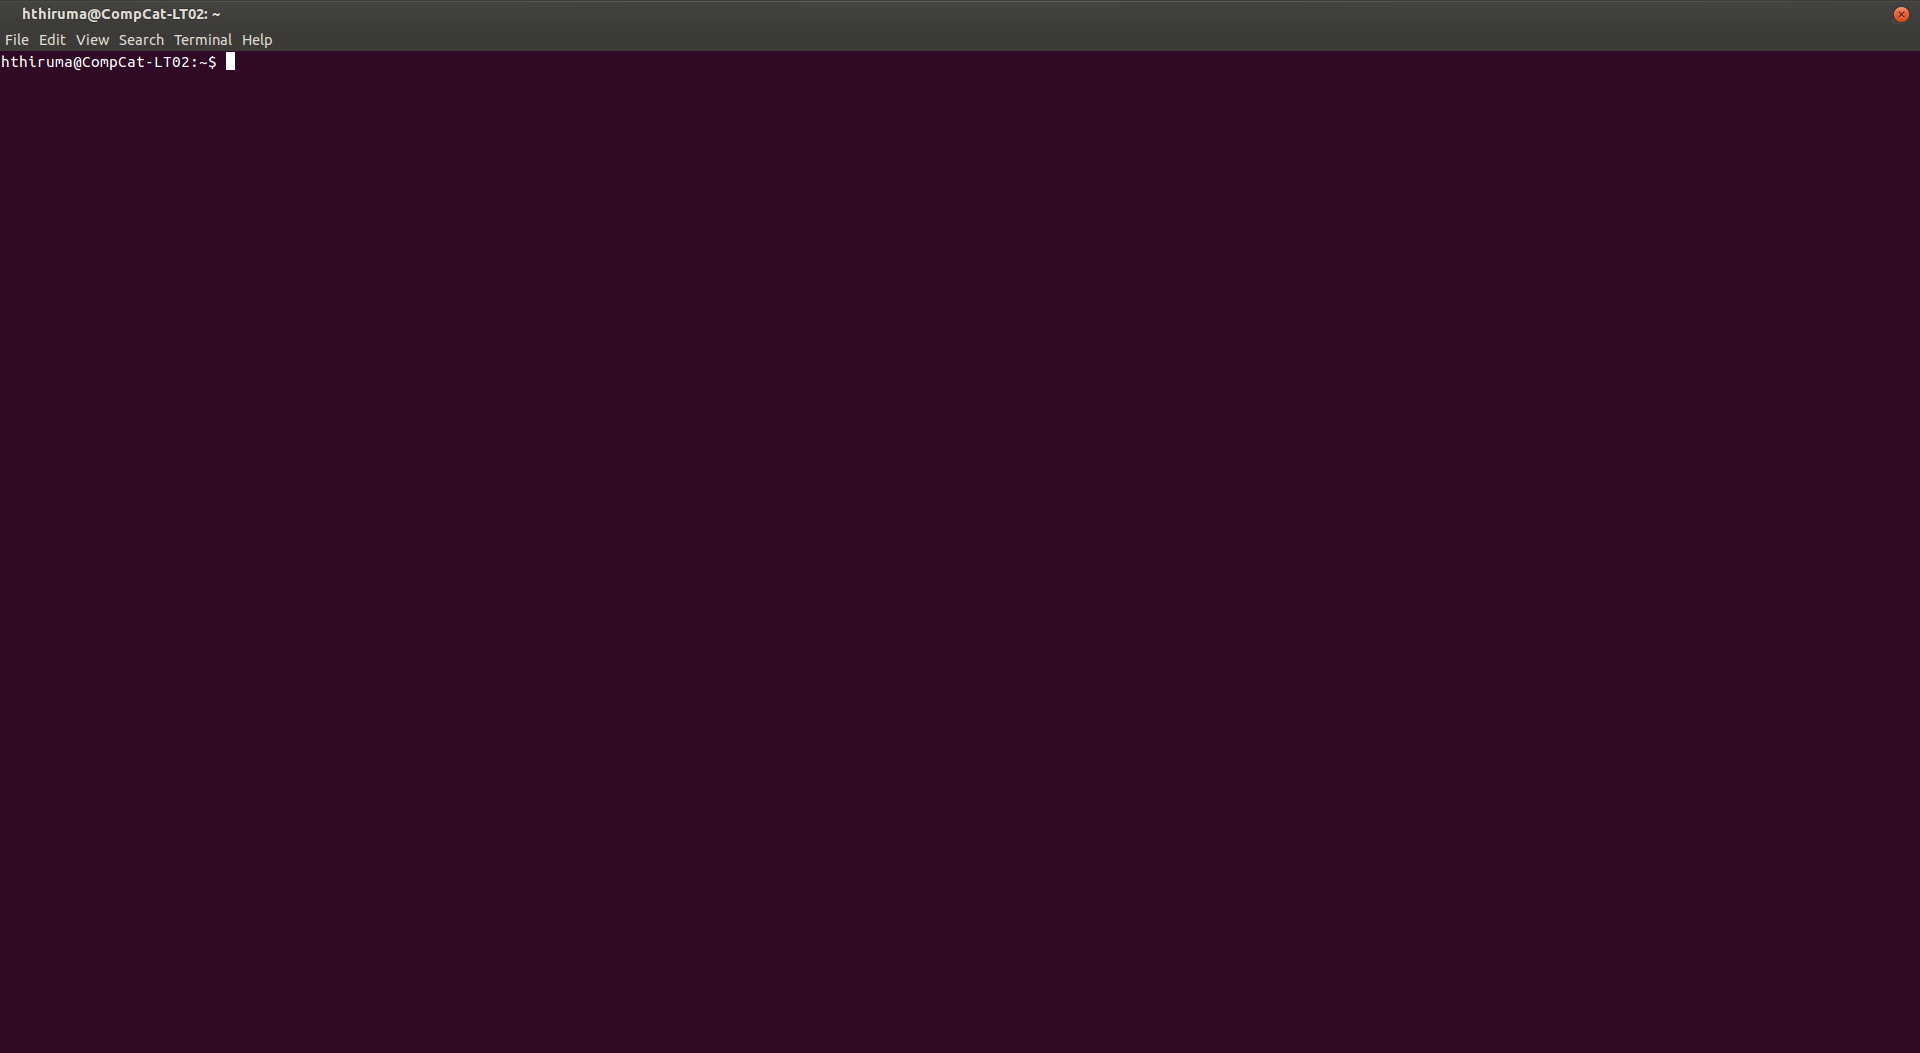
\includegraphics[width=.9\linewidth]{./figures/Ubuntu-terminal.png}
\caption{Terminal window on Linux}
\end{figure}

Windows users can install either \href{http://mobaxterm.mobatek.net/}{MobaXTerm} or \href{http://www.straightrunning.com/XmingNotes/}{Xming}. We recommend MobaXTerm.
\begin{figure}[htb]
\centering
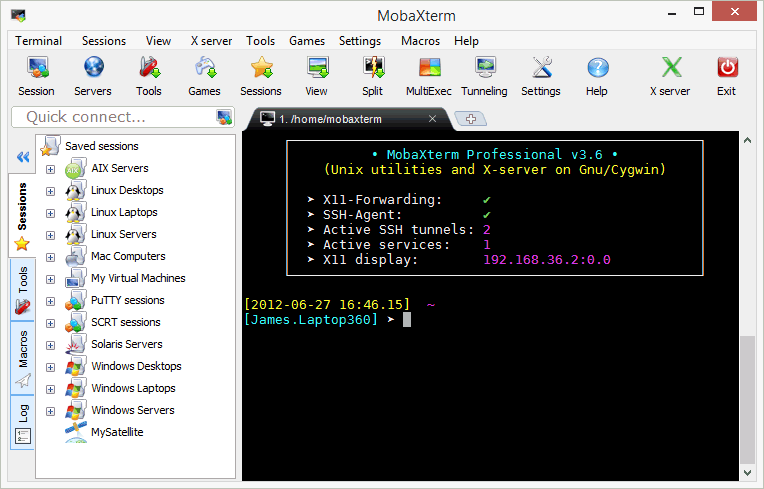
\includegraphics[width=.9\linewidth]{./figures/moba.png}
\caption{MobaXTerm Terminal window on Windows}
\end{figure}

\subsection{Logging into the cluster/supercomputer}
\label{sec-2-5}
In order to login into your account in a cluster or supercomputer you need the address of the remote machine and have an account in it. One should be able to connect to the remote computer typing the following command in a terminal
\begin{minted}[frame=lines,fontsize=\scriptsize,linenos]{sh}
ssh -X user_name@supercomputer_address
\end{minted}

Addresses of the supercomputers used by the group are:
\begin{verbatim}
System: colossus
Address: colossus.egr.uh.edu

System: opuntia
Address: opuntia.cacds.uh.edu

System: maxwell 
Address: cusco.hpcc.uh.edu

System: cori
Address: cori.nersc.gov

System: stampede2
Address: stampede2.tacc.utexas.edu

System: uhpc
Address: uhpc.hpcc.uh.edu

System: juniper
Address: juniper.hpcc.uh.edu

System: sabine
Address: sabine.cacds.uh.edu
\end{verbatim}

The environment has to be set up the first time the user logs in to load all the programs, modules and executables required for smooth functioning. This is addressed in the final section of this chapter. 

\subsection{Configuration of .cshrc file}
\label{sec-2-6}
Upon logging in to a system, there are certain default parameters and applications that will be enabled upon login and entering you terminal. The most common types of shells used are \textbf{BASH} shells and \textbf{CSH/TCSH} shells. Every shell will have a .(shell)rc file associated with it. In almost all situations, a user must modify the list of programs, defaults and executables in order to suit his or her needs. This information is stored in the \textbf{.(shell)rc} file in your system. For the clusters on campus, the defaults are setup with \textbf{CSH} shells. This file is loaded and executed every time you log in into the machine, and can be modified according to your needs.

While in your \texttt{\$HOME} directory or \textasciitilde{}/ you can access this file via \textbf{vi} editor doing:
\begin{minted}[frame=lines,fontsize=\scriptsize,linenos]{sh}
vi .cshrc
\end{minted}

Once you type \textbf{<enter>} you will be able to modify and personalize this file. This file is personal and contains some lines that configures your personal account in the cluster/supercomputer, hence, it is important to be careful with the modifications done in it.

This is how a typical \textbf{.cshrc} file looks like:
\begin{minted}[frame=lines,fontsize=\scriptsize,linenos]{sh}
module load vasp
module load ase
module load povray

setenv PATH ~/bin:/home/jarceram/apps:${PATH}

setenv DB ~/Dropbox/Post-Doc/workbooks_jmax/databases/

if ! $?PYTHONPATH then
    setenv PYTHONPATH
endif

setenv PYTHONPATH /share/apps/python2.6-extra/lib/python2.6/site-packages:${PYTHONPATH}

setenv VASPDIR '/share/apps/vasp/5.4.1/bin'
setenv VASP_COMMAND '/share/apps/openmpi-1.10.2-intel/bin/mpirun ${VASPDIR}/${VASP_EXEC}'
setenv VASP_PP_PATH /share/apps/vasp/vasp-potentials

# To create aliases, please go to the .cshrc.ext file
source ~/.cshrc.ext
\end{minted}

The user must to make sure that the enviromental variables that links VASP executables with ASE are correct and pointing to correct and accessible locations. Those variables are \textbf{VASPDIR}, \textbf{VASP\_COMMAND} and \textbf{VASP\_PP\_PATH}.

Also, depending on the cluster or supercomputer you are working on, you should be able to set helpful environmental variables by loading modules that were defined by the administrators. This is shown in the first three lines in the example \textbf{.cshrc}.

If you have doubts about what your \textbf{.cshrc}  file should contain, ask somebody in the lab, he/she will be happy to help you.


\section{Linux}
\label{sec-3}
These code blocks contain code that can be copied and pasted onto a Linux terminal or a Python interpreter, depending on the example. When using script files, you copy all lines at the once and paste them into a file that can be executed. On the other hand, if you are using the terminal or python interpreter you should copy and execute each line at a time.
\begin{minted}[frame=lines,fontsize=\scriptsize,linenos]{sh}
# First line in code 
# Second line in code
\end{minted}

The second code block that follows the first contains the expected result when executing the code in the first code block. An example of this can be seen here:
\begin{minted}[frame=lines,fontsize=\scriptsize,linenos]{python}
print (5 + 4) * (1./2)
\end{minted}

\begin{verbatim}
4.5
\end{verbatim}

\subsubsection{Basic bash shell commands}
\label{sec-3-0-1}
The commands will help you navigate through your folders, copy files, remove files and some other basic shell commands will be used in the examples of this section. 

We will start logging into one of the local clusters (Maxwell, Colossus, Opuntia or uHPC) or any other supercomputer.
\begin{minted}[frame=lines,fontsize=\scriptsize,linenos]{sh}
ssh -X user_name@supercomputer_address
\end{minted}

\begin{enumerate}
\item \textbf{mkdir}, \textbf{cd}
\label{sec-3-0-1-1}
Once in your \$HOME directory (HOME is the environmental variable that stores the path to your home directory), lets create a directory named "example" and go inside there. "\textbf{\texttt{mkdir}}" (\emph{create directory}) and "\textbf{\texttt{cd}}" (\emph{change directory}) are the commands that we need for such task
\begin{minted}[frame=lines,fontsize=\scriptsize,linenos]{sh}
mkdir example
cd example
\end{minted}
Remember that you need to type each line at a time and press \textbf{<enter>} in order to execute the command. Once you execute both lines you should be in a new empty folder.

In order to come back to the previous location (come back to the parent directory) you can use 
\begin{minted}[frame=lines,fontsize=\scriptsize,linenos]{sh}
cd ..
\end{minted}

\item \textbf{echo}, \textbf{ls}
\label{sec-3-0-1-2}
Lets know talk a little about the command "\textbf{\texttt{echo}}". This command allow you to print out text and display it in the screen. However, this simple command can also be used to write text in files in a fast way. Lets use this command in its simple form first to show you how this work:
\begin{minted}[frame=lines,fontsize=\scriptsize,linenos]{sh}
echo "Hello new member!!!"
\end{minted}

\begin{verbatim}
Hello new member!!!
\end{verbatim}

This second rectangle shows what you should observe as output in your screen. Now, go back to your previously created directory (type: \texttt{cd example}) and change the line above a little\ldots{}
\begin{minted}[frame=lines,fontsize=\scriptsize,linenos]{sh}
echo "Hello new member!!!" > hello.txt
\end{minted}

In this case the special character ">" is indicating that the text should be written in a file named "hello.txt" instead of being displayed in the screen. This means that you should now have the new file in your folder. In order to display the content of the current folder (where you currently are), you can use the command "\textbf{\texttt{ls}}".
\begin{minted}[frame=lines,fontsize=\scriptsize,linenos]{sh}
ls
\end{minted}

\begin{verbatim}
hello.txt
\end{verbatim}

"hello.txt" is now a text file located in your current position. If you want to display the content of a text file, you can use a command such as "\textbf{\texttt{more}}" followed by the file (or files) you want to display. If your file has a lot of text, then you can navigate through the text using the spacebar. To quit using the more command, press 'q'
\begin{minted}[frame=lines,fontsize=\scriptsize,linenos]{sh}
more hello.txt
\end{minted}

Now, if you want to append more lines to the same file you should use ">>". In the case you use ">" again you will erase whaterever was written in the corresponding text file.
\begin{minted}[frame=lines,fontsize=\scriptsize,linenos]{sh}
echo "This is the second line" >> hello.txt
\end{minted}
If you do more to the "hello.txt" file, you should now observe two lines as output.
\begin{minted}[frame=lines,fontsize=\scriptsize,linenos]{sh}
more hello.txt
\end{minted}

\begin{verbatim}
Hello new member!!!
This is the second line
\end{verbatim}

\item \textbf{rm}, \textbf{cp}, \textbf{mv}
\label{sec-3-0-1-3}
Remove, copy files, move or renanme files are tasks that are very often used when working with a terminal to explore and manipulate data files. Lets continue with the tutorial with these code lines in order to show you how they work.

Lets start with renaming the file you just created before "hello.txt". We will use the "\textbf{\texttt{mv}}" command to show the two main uses of this function. The first use we will show here is as rename command.
\begin{minted}[frame=lines,fontsize=\scriptsize,linenos]{sh}
mv hello.txt renamed.dat
ls
\end{minted}

Remember that with "\textbf{\texttt{ls}}" command we are showing the content of the current folder. You should see now a "rename.dat" file in your current position.
\begin{verbatim}
renamed.dat
\end{verbatim}

To move a file from one folder to another we will first create a folder called test, and move the file "renamed.dat" into that folder. 
\begin{minted}[frame=lines,fontsize=\scriptsize,linenos]{sh}
# This creates a file renamed.dat
touch renamed.dat

mkdir test
mv renamed.dat test/

ls test
\end{minted}

\begin{verbatim}
renamed.dat
\end{verbatim}

A file or folder may be copied and pasted into another file or folder of the same name, or different name using the \textbf{\texttt{cp}} command. Let us demonstrate how this can be done by copying the file "renamed.dat", from the folder \textbf{test} and into the current directory.
\begin{minted}[frame=lines,fontsize=\scriptsize,linenos]{sh}
# Copies the file renamed.dat from test/ to the current directory (.)
cp test/renamed.dat .
ls
\end{minted}

\begin{verbatim}
#dft_tutorial.org#
Icon
dft_tutorial (Copia en conflicto de Juan Manuel Arce 2016-09-01).org
dft_tutorial (Juan Manuel Arce's conflicted copy 2016-09-07).org
dft_tutorial.html
dft_tutorial.org
figures
py_ex_data.txt
renamed.dat
test
\end{verbatim}

It is also possible to copy an entire folder by using the \textbf{\texttt{cp}} command recursively. To use a command recursively, you must pass the argument \texttt{-r} along with the command. The usage of recursive copying is demonstrated below. We will try to copy the entire folder test and create another folder test-1 with the same contents
\begin{minted}[frame=lines,fontsize=\scriptsize,linenos]{sh}
cp -r test test-1
ls test
ls test-1
\end{minted}

\begin{verbatim}
renamed.dat
renamed.dat
\end{verbatim}

To remove a file or a folder, one should use the \textbf{\texttt{rm}} command as 
\begin{minted}[frame=lines,fontsize=\scriptsize,linenos]{sh}
# List contents before deletion
ls test-1

# Remove renamed.dat from test-1
rm test-1/renamed.dat

echo "Deleted"

# List contents after deletion
ls test-1

# Remove test-1 folder
# List contents of current directory
ls

rm -r test-1

# List contents of current directory after deletion
ls
\end{minted}

\begin{verbatim}
#dft_tutorial.org#
Icon
dft_tutorial (Copia en conflicto de Juan Manuel Arce 2016-09-01).org
dft_tutorial (Juan Manuel Arce's conflicted copy 2016-09-07).org
dft_tutorial.html
dft_tutorial.org
figures
py_ex_data.txt
renamed.dat
test
test-1

#dft_tutorial.org#
Icon
dft_tutorial (Copia en conflicto de Juan Manuel Arce 2016-09-01).org
dft_tutorial (Juan Manuel Arce's conflicted copy 2016-09-07).org
dft_tutorial.html
dft_tutorial.org
figures
py_ex_data.txt
renamed.dat
test
\end{verbatim}
\end{enumerate}

\subsubsection{Text editors}
\label{sec-3-0-2}
VI Editor and Emacs are commonly used text editors in the world of computing. They are similar to something familiar like Notepad in windows. Text editors are extremely important because they can open any file the contains normal ASCII text. These files can be anything from configuration files to scripts. They are very lightweight and are extremely versatile.
Both editors are fairly difficult to work with at first, and possess a steep learning curve. They are useful for different purposes, and it is best to know the basics of both, to ensure a smooth manner of working. Outside of standard tutorials, we strongly encourage you to look up resources on the internet. It has always happened that we learn something new with every new Google search. 
\begin{enumerate}
\item VI Editor
\label{sec-3-0-2-1}
vi editor is a very powerful and handy text editor used commonly by members in the group. The best way one can learn this editor is to go through the VIM Tutorial. This can be accessed on any terminal by typing 
\begin{minted}[frame=lines,fontsize=\scriptsize,linenos]{sh}
vimtutor
\end{minted}

\begin{verbatim}
=    W e l c o m e   t o   t h e   V I M   T u t o r    -    Version 1.7      =
===============================================================================

     Vim is a very powerful editor that has many commands, too many to
     explain in a tutor such as this.  This tutor is designed to describe
     enough of the commands that you will be able to easily use Vim as
     an all-purpose editor.

     The approximate time required to complete the tutor is 25-30 minutes,
     depending upon how much time is spent with experimentation.
\end{verbatim}

\item Emacs
\label{sec-3-0-2-2}
Emacs is again a very powerful and versatile text editor, used by some members (Juan Manuel and Hari) in the group. Emacs can be accessed by typing \texttt{emacs} in the terminal. In most systems, the emacs that pops up is one built into the command line, in a manner similar to the VI editor. The version of emacs used by us in the group has a graphical user interface associated with it, as well as many useful packages and functions built in. This emacs is intuitively called jmax, also the work of John Kitchin.
Emacs can be learned by opening it and accessing its tutorial on the main page.

\begin{minted}[frame=lines,fontsize=\scriptsize,linenos]{sh}
emacs
\end{minted}

\begin{figure}[htb]
\centering
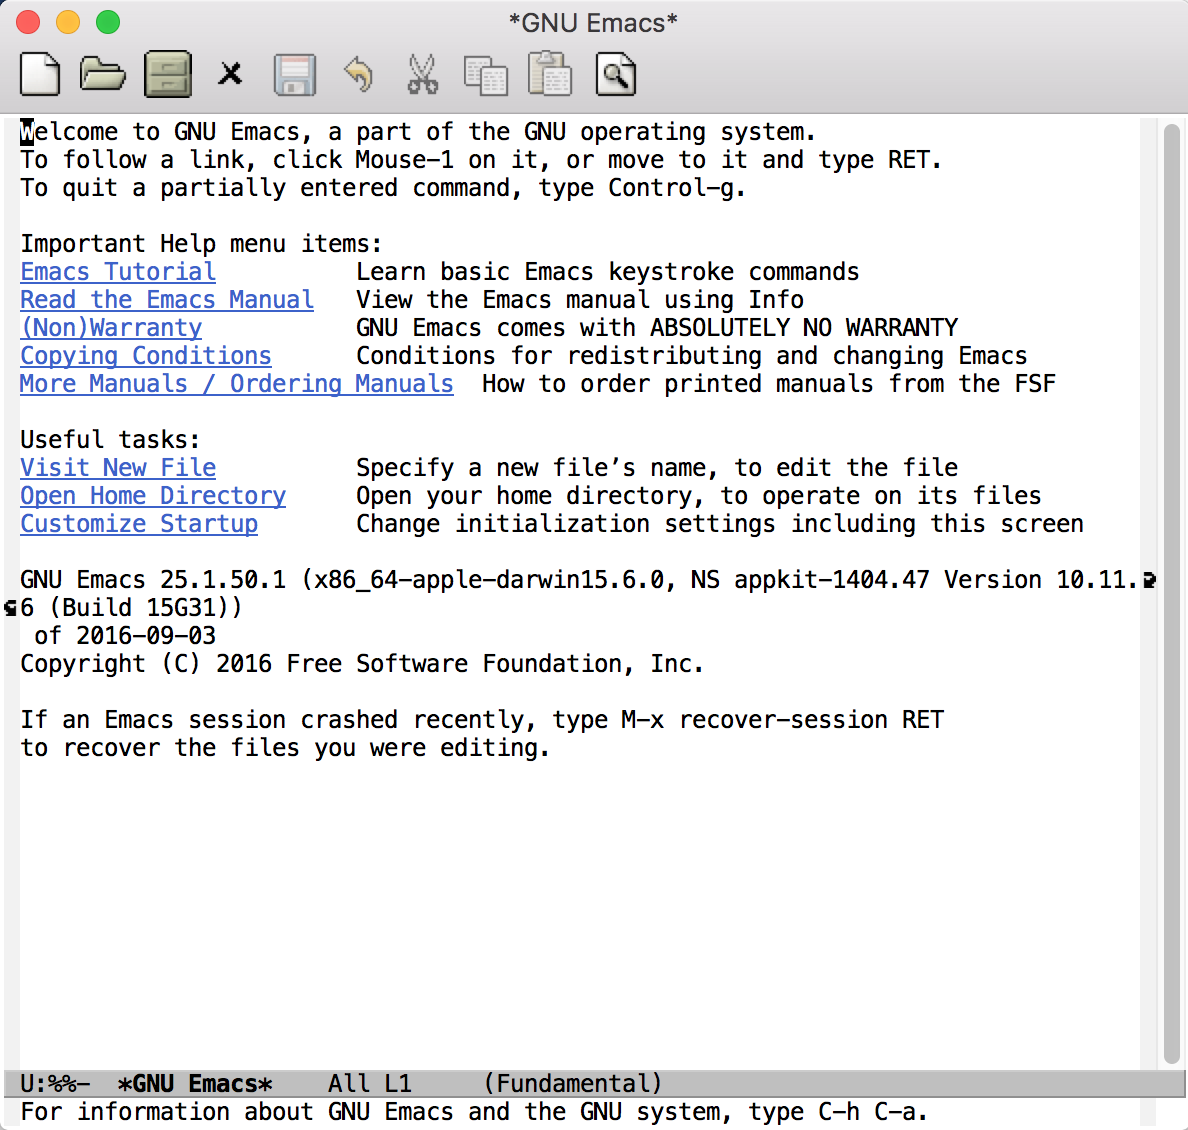
\includegraphics[width=.9\linewidth]{./figures/emacs.png}
\caption{Emacs GUI}
\end{figure}
\end{enumerate}

\section{Python}
\label{sec-4}
\subsection{Introduction}
\label{sec-4-1}
Python is a programming language which is used and documented extensively in scientific programming. We use python to interface with the Atomic Simulation Environment (ASE), which is used to build, setup and modify molecular models.
One of the best resources for learning scientific python is through \href{http://www.scipy-lectures.org/}{SciPy}, which has extensive notes and examples on using python. \href{http://kitchingroup.cheme.cmu.edu/pycse/pycse.html}{PYCSE} is a module written by \href{http://kitchingroup.cheme.cmu.edu/}{John Kitchin} and has many examples which use standard Python Modules, as well as custom modules in PYCSE. We recommend that you practise these examples as much as possible, to get a good understanding of python and how to use it to suit your needs. 
\subsection{Common used commands and basics}
\label{sec-4-2}
Even though it is impossible to be thorough in explaining in detail all commands and functions, we will show some of the most common commands and functions that you will more likely see in python scripts used for some of us in the lab. Again, we encourage you to review the broad documentation in the official webpage of \href{https://docs.python.org/2/}{Python}. 

In order to test the commands and functions you should intialize a python interpreter, with the command "python" in a linux terminal while in a computer with Python installed in it.
\subsubsection{Print}
\label{sec-4-2-1}
\begin{minted}[frame=lines,fontsize=\scriptsize,linenos]{python}
print 'Hello, this is a sample sentence!'
print 'This\tis\ttab\tseparated\ttext'
\end{minted}

\begin{verbatim}
Hello, this is a sample sentence!
This    is      tab     separated       text
\end{verbatim}

\subsubsection{Arrays and Dictionaries}
\label{sec-4-2-2}
\begin{minted}[frame=lines,fontsize=\scriptsize,linenos]{python}
import numpy as np

# Array with a range of numbers from 0 to 5, with step size of 1.
# Here, the end point is not included.
a = np.arange(0, 5, 1)
print a

# Dictionary with keys and corresponding values showing date format
b = {'Day': 'DD',
     'Month': 'MM',
     'Year': 'YYYY'}

print b
print b['Month']
\end{minted}

\begin{verbatim}
[0 1 2 3 4]
{'Year': 'YYYY', 'Day': 'DD', 'Month': 'MM'}
MM
\end{verbatim}

\subsubsection{Variable definition}
\label{sec-4-2-3}
In this section we will define 4 types of variables: string variables, scalar variables (either integer or float numbers), vector or 1-D array and matrix or 2-D array.
\begin{minted}[frame=lines,fontsize=\scriptsize,linenos]{python}
string = 'sample text'
scalar = 12
array_1d = [1,3,6,-4,0.95]
array_2d = [[1,2],[-3,2.0]]

print string 
print scalar
print array_1d
print array_2d
\end{minted}

\begin{verbatim}
sample text
12
[1, 3, 6, -4, 0.95]
[[1, 2], [-3, 2.0]]
\end{verbatim}

\subsection{Loading python modules and functions}
\label{sec-4-3}
In order to use not pre-loaded commands or functions in python you need to load them first from their modules. This means that by default Python has loaded a set of modules which contains the commands or functions that you can use right away, however, if you want to use a function that is not pre-loaded then you need to load it from the corresponding module. 

Probably the most common modules that you are going to use are these:
\begin{center}
\begin{tabular}{lll}
module & example functions & Description\\
\hline
os & mkdir, remove, getcwd, chdir & module to access operative system functionality\\
ase & Atoms & useful to handle atomic objects\\
ase.io & read, write & used to load and write atomic objects\\
ase.calculators & Vasp, Abinit & take atomic objects and calculate energies, forces, etc\\
 &  & \\
\end{tabular}
\end{center}

Modules are loaded as follows
\begin{minted}[frame=lines,fontsize=\scriptsize,linenos]{python}
import os
from ase import Atoms
from ase.io import read
from ase.calculators.vasp import Vasp
\end{minted}

\subsection{Simple data manipulation example}
\label{sec-4-4}
Data extraction and manipulation is an activity that become important, specially when dealing with huge data files or when automatization is required in order to post-process the data in an efficient way.

Lets consider that you want to determine the value of the lattice parameter of a bulk structure that minimizes the energy of the system. Do not worry to much right now in the details behind this. One approach to determine that is determining the energy of the system while changing the value of the lattice constant and then fitting the data to an equation to obtain the value that minimizes the energy. For now, we will focus in using python to extract data and manipulate them to create a simple plot. We will explain later how to determine these data points with a valid set up.

Create a text file using \textbf{vi} called py\_ex\_data.txt and copy all lines. Note that data columns are separated by tabs. 
\begin{minted}[frame=lines,fontsize=\scriptsize,linenos]{sh}
3.8	-12.28653631
3.85	-12.65124072
3.9	-12.88611724
3.95	-13.01158939
4	-13.04446413
4.05	-12.99864981
4.1	-12.88660177
4.15	-12.71939621
4.2	-12.5064955
\end{minted}

A simple code to read this file and extract the datapoints could look like the following:
\begin{minted}[frame=lines,fontsize=\scriptsize,linenos]{python}
import matplotlib.pyplot as plt

# This is only a comment. 
# Reading data file.
data = open('py_ex_data.txt','r')
lines = data.readlines()
a = []
e = []
# To go through all lines we conveniently use a FOR loop
for line in lines:
  values = line.split()
  a.append(values[0])
  e.append(values[1])

print a
print e
plt.plot(a,e,'s:k')
plt.show()
\end{minted}

\begin{verbatim}
['3.8', '3.85', '3.9', '3.95', '4', '4.05', '4.1', '4.15', '4.2']
['-12.28653631', '-12.65124072', '-12.88611724', '-13.01158939', '-13.04446413', '-12.99864981', '-12.88660177', '-12.71939621', '-12.5064955']
\end{verbatim}

Look at the four last lines, we want to display whatever were saved in the variables \textbf{a} and \textbf{e}, and we used pyplot to generate a graph with those datapoints. The resulting plot should look like the following:

\begin{figure}[htb]
\centering
\includegraphics[width=.9\linewidth]{./figures/py_ex_data.png}
\caption{Example plot}
\end{figure}

\section{Atomic Simulation Environment (ASE)}
\label{sec-5}
ASE is an Atomic Simulation Environment written in the Python programming language with the aim of setting up, steering, and analyzing atomistic simulations (adapted from \href{https://wiki.fysik.dtu.dk/ase/about.html}{ASE}). The ASE has been constructed with a number of “design goals” that make it:

\begin{itemize}
\item Easy to use:
\end{itemize}
Setting up an atomistic total energy calculation or molecular dynamics simulation with ASE is simple and straightforward. ASE can be used via a graphical user interface, Command line tools and the Python language. Python scripts are easy to follow (see What is Python? for a short introduction). It is simple for new users to get access to all of the functionality of ASE.

\begin{itemize}
\item Flexible:
\end{itemize}
Since ASE is based on the Python scripting language it is possible to perform very complicated simulation tasks without any code modifications. For example, a sequence of calculations may be performed with the use of simple “for-loop” constructions. There exist ASE modules for performing many standard simulation tasks.

\begin{itemize}
\item Customizable:
\end{itemize}
The Python code in ASE is structured in modules intended for different purposes. There are ase.calculators for calculating energies, forces and stresses, ase.md and ase.optimize modules for controlling the motion of atoms, constraints objects and filters for performing nudged-elastic-band calculations etc. The modularity of the object-oriented code make it simple to contribute new functionality to ASE.

\begin{itemize}
\item Pythonic:
\end{itemize}
It fits nicely into the rest of the Python world with use of the popular NumPy package for numerical work (see Numeric arrays in Python for a short introduction). The use of the Python language allows ASE to be used both interactively as well as in scripts.

\subsubsection{Installing ASE}
\label{sec-5-0-1}
ASE is a bundle of python modules which can be invoked or loaded when atomic simulations are required to be set up or analyzed. The easiest way of installing ase, is to download the latest source tar ball from the website. Once downloaded, the tar ball must be extracted, and installation can be completed by running 

\begin{minted}[frame=lines,fontsize=\scriptsize,linenos]{sh}
python setup.py install --user
\end{minted}

Sometimes, it is necessary to add the installation path in your \textbf{\texttt{.cshrc}} file and add \textasciitilde{}/.local/bin to the front of your PATH environment variable. This is dependent on the system you are using. 

\subsubsection{Reading and Viewing simple atoms files}
\label{sec-5-0-2}
We have downloaded a standard \texttt{cif} file (Crystallographic Information Format) from the International Zeolite Website \href{http://www.iza-online.org/}{IZA} as an example structure. The \texttt{cif} file is present as MFI.cif in this folder. 
The ASE module \texttt{ase.io} has the functions read and write which are capable of handling various formats for atomic structure, and can be used to set up every forseeable future \texttt{Vasp} calculation. An example of how to read a \texttt{cif} file is shown in the code block below.

\begin{minted}[frame=lines,fontsize=\scriptsize,linenos]{python}
# Import the read and write functions from the ase.io module.
from ase.io import read, write

# Import the visualize function to view the imported atoms object.
from ase.visualize import view

# Load the cif file into a pythonic object called 'atoms'.
atoms = read('MFI.cif')

# View the 'atoms' object.
view(atoms)
\end{minted}

Note: This jmax interface becomes inactive when you call the view function. To make it active again, close the view pop-up and then hit Ctrl+g.

\texttt{Vasp} calculations require a certain set of input files for calculation initialization. One of these files pertains to the initial structure and cartesian coordinates of the model under investigation. The name of this file is \texttt{POSCAR}. One can simply read a \texttt{cif} and write out a \texttt{POSCAR} using the functions provided by the ase.io module. An example of writing files of various formats is shown below

\begin{minted}[frame=lines,fontsize=\scriptsize,linenos]{python}
from ase.io import read, write

atoms = read('MFI.cif')

# Write the cartesian coordinates file in the =vasp= POSCAR format.
# File written in the folder 'images'
write('images/POSCAR_ZSM-5', atoms, format='vasp')

# Write the cartesian coordinates file in the =xyz= format
write('images/atoms_xyz', atoms, format='xyz')
\end{minted}

\subsubsection{Building gas phase molecules}
\label{sec-5-0-3}
Smaller models involving gas phase molecules and systems on simple surfaces are usually built up from scratch, using the modules and functions availble in ase. This can either be done through scripting or through the \texttt{ase-gui} interface. Extensive documentation on using the \texttt{ase-gui} can be accessed on the ASE website at \href{https://wiki.fysik.dtu.dk/ase/ase/gui/gui.html}{Link}. Here, we will provide a quick introduction on creating different systems.

The most simple demonstration to begin with, would be to model a simple gas phase molecule such as H$_{\text{2}}$O. ASE provides a number of ways to build and modify models, and we will explore two ways. 1) using python scripting and 2) using the ASE Graphical user interface. We recommend that you use scripting wherever possible as this keeps track of all changes made to the model, whenever documentation is necessary. 

Gas phase models are the simplest models to make, and are the least expesive in terms of computational processing time. Such systems require that they are enclosed in a vacuum cell of certain dimensions, depending on the size of the model itself. The presence and size of this cell ensures that when DFT calculations are performed, and periodic boundary conditions are implemented in X, Y and Z directions, there is minimal interaction energy between the models. Hence, one should perform calculations to ensure that energies and cell sizes are well converged, before proceeding to use data from these calculations.
We will build a simple H2O molecule in a box of 10 x 10 x 10 \AA{}. 

Note: ase.structure may have been updated to a newer version, depending on your version of ase.
\begin{minted}[frame=lines,fontsize=\scriptsize,linenos]{python}
from ase.structure import molecule
from ase.visualize import view

atoms = molecule('H2O')
atoms.set_cell([10, 10, 10])
atoms.center()

view(atoms)
\end{minted}

\begin{figure}[htb]
\centering
\includegraphics[width=.9\linewidth]{./figures/molec_h2o_ase_ex.png}
\caption{H$_{\text{2}}$O molecule in a box}
\end{figure}

As you can see we have used the "molecule" and "view" functions from the "structure" and "visualize" subpackages in order to build and visualize the molecule. Again, you need to load modules and subpackages in order to use installed/non-default python packages.

\begin{minted}[frame=lines,fontsize=\scriptsize,linenos]{python}
# From the Atoms and Atom modules
from ase import Atom, Atoms
from ase.visualize import view
from ase.io import read, write

# Creating a random model with H, O and C at random positions
atoms = Atoms([Atom('H', [0, 0, 0]),
               Atom('O', [1, 1, 1]), 
               Atom('C', [2, 2, 1])])

# Set a cell of dimensions 10 \AA
atoms.set_cell([10, 10, 10])
write('images/not-centered.png', atoms, show_unit_cell=True)
# The atoms and the cell originate at [0, 0, 0], and the model will not be centered within the cell
# it is important to center the model so that there is equal vacuum on all sides.
atoms.center()

write('images/centered.png', atoms, show_unit_cell=True)
write('images/POSCAR_random', atoms, format='vasp')
\end{minted}

\subsubsection{Building crystal structures}
\label{sec-5-0-4}
Crystals are materials that maintain an order in a microscopic scale and in all three dimensions. In other words, the building block (unit cell) of a crystalline material is repeated in the 3-dimensional space, or it is isotropic. Take for instance the example shown in the following figure in which we are displaying the structure of the rutile crystal phase of TiO$_{\text{2}}$ (rut-TiO$_{\text{2}}$). In this figure, the dashed-line box represent the limits of the unit cell that is repeated in all directions.

\begin{figure}[htb]
\centering
\includegraphics[width=.9\linewidth]{./figures/rut-TiO2_ex.png}
\caption{Crystal structure of rutile-TiO$_{\text{2}}$}
\end{figure}

One way to build a crystal structure through ASE is the "spacegroup" subpackage. This subpackage requires that you to provide the crystal space group, the lattice parameters and the scaled positions of the unique atoms (the number of atoms provided not necessarily match with the number of atoms in the unit cell). Lets continue with the example of rut-TiO$_{\text{2}}$ and try to build the same crystal structure. We will need detailed information about this crystal that can be found in scientific articles or databases. An example of python script to carry out the task can look like the following:

\begin{minted}[frame=lines,fontsize=\scriptsize,linenos]{python}
from ase.lattice.spacegroup import crystal
from ase.visualize import view

# Lattice parameters. Experimetnal values for TiO2 rutile
a = 4.5937
c = 2.9587

# Using the 'crystal' function from 'spacegroup' subpackage
# Data provided (in order of appearence)
# Unique atoms in unit cell; scaled positions of unique atoms;
# Space group ID #; dimension of unit cell (lattice param. and angles)
rut = crystal(['Ti','O'], basis=[(0.0,0.0,0.0),(0.3048,0.3048,0.0)],
   spacegroup=136, cellpar=[a, a, c, 90, 90, 90])

view(rut)
\end{minted}

\begin{figure}[htb]
\centering
\includegraphics[width=.9\linewidth]{./figures/rut-TiO2_ase_ex.png}
\caption{Output after running the previous python script that builds rut-TiO$_{\text{2}}$}
\end{figure}

As you can see from what was displayed through ASE graphical user interface, the unit cell of rut-TiO$_{\text{2}}$ contains two Ti and four O atoms, however, we only specified two positions in the script. This is why we need to provide the space group, in order to let know ASE where the other equivalent atoms should be placed according to symmetric positions that are dependent of the space group.

Even though you can provide of very reliable experimental information, the atomic positions and cell size and shape usually need to be computationally optimized before can be used to generate a surface or for energy comparisons. We will talk later about a method that can be used to optimize a crystal structure.  

\subsubsection{Building surfaces}
\label{sec-5-0-5}
If you want to simulate the adsorption of a chemical compounds and its interaction with a solid catalyst, you might want to create a representative model of the solid in question. Here, we explain how to create a surface model that could be used for following calculations, such adsorption tests. 

We will build a slab of the (101) exposed facet of tetragonal zirconium oxide from its crystal structure parameters. First, you will need the lattice parameters required to build a bulk crystal (as was done for rut-TiO2 above). The lattice parameters are shown in the piece of code below, together with an extra line with the function "surface" that can be used to build a surface from a bulk crystal model. In this case, the function needs a atoms object ("atoms", here in the code), the plane at which the cut should be done, the number of layers that should be included and the length of the vacuum layer in each side of slab (in angstroms). 

\begin{minted}[frame=lines,fontsize=\scriptsize,linenos]{python}
from ase.lattice.spacegroup import crystal
from ase.visualize import view
from ase.lattice.surface import surface

a = 3.63
c = 5.25
z = 0.05

atoms = crystal(['Zr', 'O'], basis=[(0.0, 0.0, 0.0), (0.0, 0.5, z+0.25)],
   spacegroup=137, cellpar=[a, a, c, 90, 90, 90])

surface = surface(atoms, (1,0,1), 5, 7.5)
view(surface)
\end{minted}

\begin{figure}[htb]
\centering
\includegraphics[width=.9\linewidth]{./figures/ZrO2_surf_ex.png}
\caption{Slab of t-ZrO2 (101) built from bulk.}
\end{figure}

Even though this procedure is very simple, one needs to be really careful in the selection of the surface termination. For instance, by looking at the slab generated by ASE one can see that the exposed surface in +z direction has a oxygen termination, that might not be (and is not) the most stable termination. However, by deleting this "extra" oxygen atoms on top, we are also changing the Zr/O ratio. The surface slab is now no longer stoichiometric (Zr$_{\text{10}}$O$_{\text{18}}$ instead of Zr$_{\text{10}}$O$_{\text{20}}$). Is usually a good idea to keep the stoichiometry in order to avoid strong polarization (\#\#is this right??). This is usually not a problem for simple metal surfaces that are highly symetrical or are built by only one distinguishable metal.

One way to solve this problem can be creating a slab with an extra layer and then deleting the atoms that are not longer needed in order to maintain the desirable number of layers. At the end, is possible that we need to shift the position of all atoms in the cell in order to keep the center of mass in the center of the cell. We are going to use a similar script to create a slab with an extra layer and then delete some of the atoms, so we keep only 5 layers in total.

\begin{minted}[frame=lines,fontsize=\scriptsize,linenos]{python}
from ase.lattice.spacegroup import crystal
from ase.visualize import view
from ase.lattice.surface import surface

a = 3.63
c = 5.25
z = 0.05

atoms = crystal(['Zr', 'O'], basis=[(0.0, 0.0, 0.0), (0.0, 0.5, z+0.25)],
   spacegroup=137, cellpar=[a, a, c, 90, 90, 90])

surface = surface(atoms, (1,0,1), 6, 7.5)

# Lets remove the atoms that should lead to a 5-layered non-oxygen terminated stoichiometric surface
ind2remove = [0,1,2,5,33,34]
for i in sorted(ind2remove, reverse=True):
   del surface[i]

# Tranlate atoms to the new center
cell = surface.get_cell()
com = surface.get_center_of_mass()
surface.translate([0,0,0.5*cell[2,2] - com[2]])

view(surface)
\end{minted}

As a result, you should get a new slab with the right termination but also one that keeps the Zr/O ratio to 1/2. As you can see in the script we have removed some of the atoms (indicating their indixes in the atomic object) and we shift the position of the whole slab in the z-direction so the center of mass of the slab resides again in the center of the cell.

We now can use this slab for following calculations.  

\subsubsection{Get details of an atoms object}
\label{sec-5-0-6}
ASE has many useful functions, which when used efficiently are very powerful in automating scripts and workflow. Given that we have already learned to build complex models and structures, we must also know how to extract details from atoms objects, in the case of analysis and post-processing. Examples of simple ase functions for this purpose are shown below.
\begin{minted}[frame=lines,fontsize=\scriptsize,linenos]{python}
from ase.io import read

# Read atoms from previously stored POSCAR
atoms = read('images/POSCAR_ZSM-5')

# Get unit cell parameters
cell = atoms.get_cell()
print 'Unit cell array:' 
print cell, '\n'

# Get details of all individual atoms making up the entire atoms object
# Printing only first 10 atom details, using python list indexing
print('Details of 10 individual atoms: ')
for atom in atoms[0:10]:
    print atom

# Get positions of atoms, and print specific details
positions = atoms.get_positions()

# Using python string formatting and enumeration concepts
print('\nAtom specific details: ')
for i, atom in enumerate(atoms[0:10]):
    print('Index: {0}, Element: {1}, Coordinates: {2}'.format(i, atom.symbol, positions[i]))
\end{minted}

\begin{minted}[frame=lines,fontsize=\scriptsize,linenos]{sh}
Unit cell array:
[[  2.00900000e+01   0.00000000e+00   0.00000000e+00]
 [  1.20000000e-15   1.97380000e+01   0.00000000e+00]
 [  8.00000000e-16   8.00000000e-16   1.31420000e+01]] 

Details of 10 individual atoms: 
Atom('O', [10.069108, 1.3796862000000008, 9.2230555999999986], index=0)
Atom('O', [20.065892000000002, 11.2486862, 2.6520555999999997], index=1)
Atom('O', [10.069108, 8.4893137999999997, 9.2230555999999986], index=2)
Atom('O', [20.065892000000002, 18.358313800000001, 2.6520555999999997], index=3)
Atom('O', [10.020892000000002, 18.358313800000001, 3.9189444], index=4)
Atom('O', [0.024107999999998499, 8.4893137999999997, 10.489944400000001], index=5)
Atom('O', [10.020892, 11.2486862, 3.9189444], index=6)
Atom('O', [0.0241079999999981, 1.3796862000000008, 10.489944400000001], index=7)
Atom('O', [7.7848750000000013, 1.4665334000000008, 10.5241136], index=8)
Atom('O', [2.2601250000000013, 11.335533400000001, 3.9531135999999991], index=9)

Atom specific details: 
Index: 0, Element: O, Position: [ 10.069108    1.3796862   9.2230556]
Index: 1, Element: O, Position: [ 20.065892   11.2486862   2.6520556]
Index: 2, Element: O, Position: [ 10.069108    8.4893138   9.2230556]
Index: 3, Element: O, Position: [ 20.065892   18.3583138   2.6520556]
Index: 4, Element: O, Position: [ 10.020892   18.3583138   3.9189444]
Index: 5, Element: O, Position: [  0.024108    8.4893138  10.4899444]
Index: 6, Element: O, Position: [ 10.020892   11.2486862   3.9189444]
Index: 7, Element: O, Position: [  0.024108    1.3796862  10.4899444]
Index: 8, Element: O, Position: [  7.784875    1.4665334  10.5241136]
Index: 9, Element: O, Position: [  2.260125   11.3355334   3.9531136]
\end{minted}

\subsubsection{Edit a loaded atoms object}
\label{sec-5-0-7}
Pre-loaded atoms objects can be edited to suit the requirements of the model, and other constraints. The process of editing is simple. First, the relevant model (POSCAR or cif) is loaded. Specific details like position can be obtained using relevant functions. Modifications to these details are then made, and finally, the modifications are implemented in the atoms object using relevant functions. An example follows.

\begin{minted}[frame=lines,fontsize=\scriptsize,linenos]{python}
from ase.io import read

atoms = read('images/POSCAR_ZSM-5')

# Store required atom into a new variable.
# Note: This is usually done in less explicit ways
atom = atoms[4]
positions = atoms.get_positions()

# Printing coordinates before implementing changes
print 'Coordinates of atom number 4: ', atom.position
print 'Element of atom number 4: ', atom.symbol

# We want to change the element and cartesian coordinates of the atom with index=4.
positions[4] = [1, 1, 1]
atoms[4].symbol = 'C'

# Reassign modified positions to original atoms object
atoms.set_positions(positions)

print '\nDetails after implementing changes: '
atom = atoms[4]
print 'Coordinates of atom number 4: ', atom.position
print 'Element of atom number 4: ', atom.symbol
\end{minted}

\begin{verbatim}
Coordinates of atom number 4:  [ 10.020892   18.3583138   3.9189444]
Element of atom number 4:  O

Details after implementing changes: 
Coordinates of atom number 4:  [ 1.  1.  1.]
Element of atom number 4:  C
\end{verbatim}

\subsubsection{Adding Atoms to Existing Model}
\label{sec-5-0-8}
The atoms object is essentially a python list of individual atoms objects. Hence, one can perform the same operations on atoms objects as simple lists. New atoms can be added to an existing atoms object using the append function in python. However, if you want to add an entire atoms object to a pre-existing atoms object, then one must use the python extend function. Please read up the differences between append() and extend() for better clarity
In the example shown below, both atoms objects end up identical.

\begin{minted}[frame=lines,fontsize=\scriptsize,linenos]{python}
from ase.io import read
from ase import Atom, Atoms

# Read in two pre-existing atoms objects
atoms = read('images/POSCAR_ZSM-5')
atoms_new = read('images/POSCAR_random')

# Generate a copy of the original atoms object
atoms1 = atoms.copy()

# To add atoms_new to atoms, we use the extend() function
atoms1.extend(atoms_new)
print atoms1

# Define explicit atom objects
H = Atom('H', [0, 0, 0])
O = Atom('O', [1, 1, 1]) 
C = Atom('C', [2, 2, 1])

# Generate a copy of the original atoms object
atoms2 = atoms.copy()

# Use the append() function to individually append the atom objects to the atoms object
atoms2.append(H)
atoms2.append(O)
atoms2.append(C)

print atoms2
\end{minted}

\begin{verbatim}
Atoms(symbols='CHO193Si96', positions=..., cell=[[20.09, 0.0, 0.0], [1.2e-15, 19.738, 0.0], [7.9999999999999998e-16, 7.9999999999999998e-16, 13.141999999999999]], pbc=[True, True, True])
Atoms(symbols='CHO193Si96', positions=..., cell=[[20.09, 0.0, 0.0], [1.2e-15, 19.738, 0.0], [7.9999999999999998e-16, 7.9999999999999998e-16, 13.141999999999999]], pbc=[True, True, True])
\end{verbatim}

\section{Setting up and Submitting a VASP Calculation}
\label{sec-6}
\subsection{Quick Introduction to VASP}
\label{sec-6-1}
Having introduced how to set up a model, and high performance computing concepts, we can now proceed towards setting up and submitting a VASP Calculation.

The Vienna ab initio Simulation Package or (\href{https://www.vasp.at/}{VASP}) is a code that implements Density Functional Theory concepts to perform energy minimization to obtain the ground state atomic configuration of the model under investigation. \texttt{VASP} is installed on all of our supercomputers and can be invoked by loading the relevant modules. Currently installed \texttt{VASP} versions are 5.3.5 and 5.4.1. There is no performance benefit of using one over the other. It is a matter of your choice. Calculation times are dependent on the size of the system, and more specifically, the number of electrons. Calculations for small systems converge to their ground states very quickly. However large systems may sometimes run for many weeks. It is for this reason that \texttt{VASP} is run parallely across many processors or nodes. A system utility named \texttt{mpirun} is responsible for the execution of \texttt{VASP} on massively parallel systems, such as ours.

A standard \texttt{VASP} calculation, in short, requires 4 files to initiate a calculation
\begin{itemize}
\item POSCAR - This file contains the cartesian coordinates, type and number of species present in the model.
\item INCAR - This file consists of the calculation parameters required by \texttt{VASP}.
\item KPOINTS - This file specifies the type of grid required for calculations.
\item POTCAR - This file contains the reference pseudopotentials required for calculations.
\end{itemize}

This is just a cursory introduction to the files used by \texttt{VASP}. It is recommended for you to go through and understand the \texttt{VASP} manual and other online resources for a better understanding \href{https://www.vasp.at/index.php/documentation}{Link}. 

\subsection{Using ASE to Set Up a Calculation}
\label{sec-6-2}
Again, ASE has many functions and methods which can be used to set up the entire \texttt{VASP} calculation through python. Let us recall that we already learnt how to set up the model through python by the generation of atoms objects \texttt{POSCAR}. The \texttt{INCAR} is automatically set up by ase when a \textbf{Vasp calculator object} is used. The user can enter values for calculator parameters in this object, and also other specifc triggers to write the \texttt{KPOINTS} and \texttt{POTCAR} files. A simple example follows

\begin{minted}[frame=lines,fontsize=\scriptsize,linenos]{python}
# Import the vasp calculator object
from ase.calculators.vasp import Vasp

# Read in the cif file, or a pre-made atoms object
atoms = read('images/MFI.cif')

# Define the calculator and its parameters
calc = Vasp(xc='PBE',  # Exchange Correlation Functional
            encut=400, # Plane Wave Cutoff
            ibrion=2,  # Energy Minimization Algorithm
            kpts=(2,2,2), # K-point grid. Writes KPOINTS FILE
            ediffg=0.02, # Iterative Convergence Criteria
            nsw=500) # Maximum number of Iterations

# Set the calculator to the atoms object
atoms.set_calculator(calc)
\end{minted}

The snippet of code shown above creates all the files required by \texttt{VASP}. Creation of files is done in the following manner. First, the calculator stores information about the model, the elements, the stoichiometry and the cartesian coordinates. Based on the calculator parameters written in by the user, and combining them with defaults, it stores the entire list of parameters and creates the \texttt{INCAR} file. Based on the parameters, and the type of atoms, it creates the \texttt{POTCAR} and \texttt{KPOINTS} files. Finally, the user is free to call vasp at his or her convenience. 

\subsection{Executing the Calculation}
\label{sec-6-3}
We have created all required files for a calculation. The next course of action is to invoke \texttt{VASP}. This is usually done by setting an \href{https://en.wikipedia.org/wiki/Environment_variable}{Environment Variable} called 'VASP\_EXEC' in your jobscript. When you submit your jobscript to the queue, it will load the specific \texttt{VASP} specified by you in this environment variable. A simple jobscript, assuming that the cif file is in the same folder, is shown below

\begin{minted}[frame=lines,fontsize=\scriptsize,linenos]{python}
#!/usr/bin/env python

#PBS -e stderr
#PBS -o stdout
#PBS -m ae
#PBS -M hthirumalai@gmail.com
#PBS -l walltime=100:00:00
#PBS -r n
#PBS -l nodes=1:ppn=12
#PBS -l pmem=2500mb
#PBS -S /bin/tcsh
#PBS -V

from ase.io import read
from ase.calculators.vasp import Vasp

atoms = read('MFI.cif')

calc = Vasp(xc='PBE',
            encut=540,
            ibrion=2,
            sigma=0.1,
            ediffg=-0.02,
            nsw=500)

atoms.set_calculator(calc)
e = atoms.get_potential_energy()

f = open('energy', 'w')
f.write(str(e))
f.close()
\end{minted}
% Emacs 26.0.50 (Org mode 8.2.10)
\end{document}